\section{The Mean Value Theorem for Integrals and Average Value}{}{}\label{sec:Average Value}


\begin{figure}[H]
\begin{tikzpicture}
\begin{axis}[width=\marginparwidth+25pt,%
tick label style={font=\scriptsize},axis y line=middle,axis x line=middle,name=myplot,axis on top,%
			%x=.37\marginparwidth,
			%y=.37\marginparwidth,
			xtick={1,2,3,4},% 
%			extra x ticks={.5,3},
%			extra x tick labels={$a$,$b$},
			ytick=\empty,
			%minor y tick num=1,%extra y ticks={-5,-3,...,7},%
%			minor x tick num=4,
			ymin=-.5,ymax=1.75,%
			xmin=-.5,xmax=4.5%
]
\addplot [smooth,thick, {red},domain=-.5:4.5] {.3*cos(deg(x))+1}; 
\end{axis}

\node [right] at (myplot.right of origin) {\scriptsize $x$};
\node [above] at (myplot.above origin) {\scriptsize $y$};
\end{tikzpicture}
\caption{A graph of a function $f$ to introduce the Mean Value Theorem.\label{fig:ftc7a}} 
\end{figure}

Consider the graph of a function $f$ in Figure \ref{fig:ftc7a} and the area defined by $\int_1^4 f(x)\ dx$. Three rectangles are drawn in Figure \ref{fig:ftc7b}; in (a), the height of the rectangle is greater than $f$ on $[1,4]$, hence the area of this rectangle is is greater than $\int_0^4 f(x)\ dx$. 

In (b), the height of the rectangle is smaller than $f$ on $[1,4]$, hence the area of this rectangle is less than $\int_1^4 f(x)\ dx$.


\begin{figure}[H]
\begin{subfigure}{.33\textwidth}
\begin{tikzpicture}
\begin{axis}[width=\marginparwidth+25pt,%
tick label style={font=\scriptsize},axis y line=middle,axis x line=middle,name=myplot,axis on top,%
			%x=.37\marginparwidth,
			%y=.37\marginparwidth,
			xtick={1,2,3,4},% 
%			extra x ticks={.5,3},
%			extra x tick labels={$a$,$b$},
			ytick=\empty,
			%minor y tick num=1,%extra y ticks={-5,-3,...,7},%
%			minor x tick num=4,
			ymin=-.5,ymax=1.75,%
			xmin=-.5,xmax=4.5%
]

\addplot [{green},thick,fill={green},domain=1:4] {.3*cos(deg(x))+1} \closedcycle;
\addplot [smooth,thick, {green},domain=-.5:4.5] {.3*cos(deg(x))+1}; 
\draw [thick,draw={red}] (axis cs: 1,0) rectangle (axis cs:4,.65);
\end{axis}

\node [right] at (myplot.right of origin) {\scriptsize $x$};
\node [above] at (myplot.above origin) {\scriptsize $y$};
\end{tikzpicture}
\caption{}
  \label{fig:ftc7a}
\end{subfigure}%
\begin{subfigure}{.33\textwidth}
\begin{tikzpicture}
\begin{axis}[width=\marginparwidth+25pt,%
tick label style={font=\scriptsize},axis y line=middle,axis x line=middle,name=myplot,axis on top,%
			%x=.37\marginparwidth,
			%y=.37\marginparwidth,
			xtick={1,2,3,4},% 
%			extra x ticks={.5,3},
%			extra x tick labels={$a$,$b$},
			ytick=\empty,
			%minor y tick num=1,%extra y ticks={-5,-3,...,7},%
%			minor x tick num=4,
			ymin=-.5,ymax=1.75,%
			xmin=-.5,xmax=4.5%
]

\addplot [{green},thick,fill={green},domain=1:4] {.3*cos(deg(x))+1} \closedcycle;
\addplot [smooth,thick, {\colorone},domain=-.5:4.5] {.3*cos(deg(x))+1}; 
\draw [thick,draw={\colortwo}] (axis cs: 1,0) rectangle (axis cs:4,1.35);
\end{axis}

\node [right] at (myplot.right of origin) {\scriptsize $x$};
\node [above] at (myplot.above origin) {\scriptsize $y$};
\end{tikzpicture}
\caption{}
  \label{fig:ftc7b}
\end{subfigure}%
\begin{subfigure}{.33\textwidth}
\begin{tikzpicture}
\begin{axis}[width=\marginparwidth+25pt,%
tick label style={font=\scriptsize},axis y line=middle,axis x line=middle,name=myplot,axis on top,%
			%x=.37\marginparwidth,
			%y=.37\marginparwidth,
			xtick={1,2,3,4},% 
%			extra x ticks={.5,3},
%			extra x tick labels={$a$,$b$},
			ytick=\empty,
			%minor y tick num=1,%extra y ticks={-5,-3,...,7},%
%			minor x tick num=4,
			ymin=-.5,ymax=1.75,%
			xmin=-.5,xmax=4.5%
]

\addplot [{green},thick,fill={green},domain=1:4] {.3*cos(deg(x))+1} \closedcycle;
\addplot [smooth,thick, {\colorone},domain=-.5:4.5] {.3*cos(deg(x))+1}; 
\draw [thick,draw={\colortwo}] (axis cs: 1,0) rectangle (axis cs:4,.84);
\end{axis}

\node [right] at (myplot.right of origin) {\scriptsize $x$};
\node [above] at (myplot.above origin) {\scriptsize $y$};
\end{tikzpicture}

\caption{}
  \label{fig:ftc7c}
\end{subfigure}%
\caption{Differently sized rectangles give upper and lower bounds on $\int_1^4 f(x)\ dx$; the last rectangle matches the area exactly.\label{fig:ftc7}} 
\end{figure}


Finally, in (c) the height of the rectangle is such that the area of the rectangle is \textit{exactly} that of $\int_0^4 f(x)\ dx$. Since rectangles that are ``too big\primeskip'', as in (a), and rectangles that are ``too little,'' as in (b), give areas greater/lesser than $\int_1^4 f(x)\ dx$, it makes sense that there is a rectangle, whose top intersects $f(x)$ somewhere on $[1,4]$, whose area is \textit{exactly} that of the definite integral.


We state this idea formally in a theorem.

\begin{theorem}{The Mean Value Theorem of Integration}{mvt2}
{Let $f$ be continuous on $[a,b]$.\index{Mean Value Theorem!of integration}\index{integration!Mean Value Theorem} There exists a value $c$ in $[a,b]$ such that $$\int_a^bf(x)\ dx = f(c)(b-a).$$
}
\end{theorem}

This is an \emph{existential} statement; $c$ exists, but we do not provide a method of finding it. Theorem \ref{thm:mvt2} is directly connected to the Mean Value Theorem of Differentiation, given %in Section \ref{sec:mvt} 
as Theorem \ref{thm:mvt}; we leave it to the reader to see how.

We demonstrate the principles involved in this version of the Mean Value Theorem in the following example.\\


\begin{example}{Using the Mean Value Theorem}{ex_ftc8}
{
Consider $\int_0^\pi \sin x\ dx$. Find a value $c$ guaranteed by the Mean Value Theorem.
}
\end{example}

\begin{solution}
{We first need to evaluate $\int_0^\pi \sin x\ dx$. (This was previously done in Example \ref{ex_ftc4}.)
		$$\int_0^\pi\sin x\ dx =	-\cos x \Big|_0^\pi = 2.$$
Thus we seek a value $c$ in $[0,\pi]$ such that $\pi\sin c =2$. 
$$\pi\sin c = 2\ \ \Rightarrow\ \ \sin c = 2/\pi\ \ \Rightarrow\ \ c = \arcsin(2/\pi) \approx 0.69.$$

\begin{figure}[H]
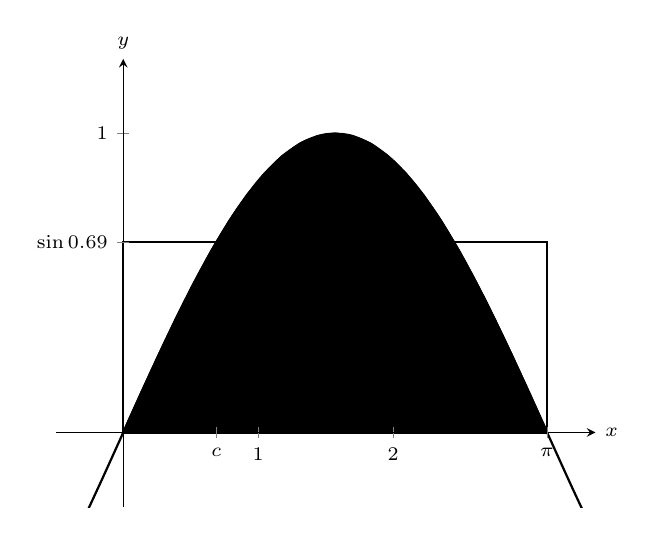
\begin{tikzpicture}
\begin{axis}[ %width=\marginparwidth+25pt,%
tick label style={font=\scriptsize},axis y line=middle,axis x line=middle,name=myplot,axis on top,%
			%x=.37\marginparwidth,
			%y=.37\marginparwidth,
			xtick={1,2},% 
			extra x ticks={.69,3.14},
			extra x tick labels={$c$,$\pi$},
			ytick={1},
			%minor y tick num=1,
			extra y ticks={.637},%
			extra y tick labels={$\sin 0.69$},
%			minor x tick num=4,
			ymin=-.25,ymax=1.25,%
			xmin=-.5,xmax=3.5%
]

\addplot [{\coloronefill},thick,fill={\coloronefill},domain=0:3.14] {sin(deg(x))} \closedcycle;
\addplot [smooth,thick, {\colorone},domain=-.5:3.5] {sin(deg(x))}; 
\draw [thick,draw={\colortwo}] (axis cs: 0,0) rectangle (axis cs:3.14,.637);
\end{axis}

\node [right] at (myplot.right of origin) {\scriptsize $x$};
\node [above] at (myplot.above origin) {\scriptsize $y$};
\end{tikzpicture}
\caption{A graph of $y=\sin x$ on $[0,\pi]$ and the rectangle guaranteed by the Mean Value Theorem. \label{fig:ftc8}} 
\end{figure}


In Figure \ref{fig:ftc8} $\sin x$ is sketched along with a rectangle with height $\sin (0.69)$. The area of the rectangle is the same as the area under $\sin x$ on $[0,\pi]$.
}\\
\end{solution}

Let $f$ be a function on $[a,b]$ with $c$ such that $f(c)(b-a) = \int_a^bf(x)\ dx$. Consider $\int_a^b\big(f(x)-f(c)\big)\ dx$:
\begin{align*}
	\int_a^b\big(f(x)-f(c)\big)\ dx &=	\int_a^b f(x) - \int_a^b f(c)\ dx\\
							&= f(c)(b-a) - f(c)(b-a) \\
							&= 0.
\end{align*}
When $f(x)$ is shifted by $-f(c)$, the amount of area under $f$ above the $x$--axis on $[a,b]$ is the same as the amount of area below the $x$--axis above $f$; see Figure \ref{fig:ftc9} for an illustration of this. In this sense, we can say that $f(c)$ is the \textit{average value} of $f$ on $[a,b]$. 






\begin{figure}[H]
\begin{subfigure}{.5\textwidth}
\begin{tikzpicture}
\begin{axis}[width=\marginparwidth+25pt,%
tick label style={font=\scriptsize},axis y line=middle,axis x line=middle,name=myplot,axis on top,%
			%x=.37\marginparwidth,
			%y=.37\marginparwidth,
			xtick=\empty,% 
			extra x ticks={1,4,1.63},
			extra x tick labels={$a$,$b$,$c$},
			ytick=\empty,
			%minor y tick num=1,
			extra y ticks={1.75},%
			extra y tick labels={$f(c)$},
%			minor x tick num=4,
			ymin=-1,ymax=3.5,%
			xmin=-.5,xmax=4.25%
]

\addplot [{\coloronefill},thick,fill={\coloronefill},domain=1:4] {(x-2.5)^2+1} \closedcycle;
\addplot [smooth,thick, {\colorone},domain=-.5:4.25] {(x-2.5)^2+1}; 
\draw [thick,draw={\colortwo}] (axis cs: 1,0) rectangle (axis cs:4,1.75);
\draw (axis cs:3.35,3) node {\scriptsize $y=f(x)$};
\end{axis}

\node [right] at (myplot.right of origin) {\scriptsize $x$};
\node [above] at (myplot.above origin) {\scriptsize $y$};
\end{tikzpicture}



\caption{}
  \label{fig:ftc9a}
\end{subfigure}%
\begin{subfigure}{.5\textwidth}
\begin{tikzpicture}
\begin{axis}[width=\marginparwidth+25pt,%
tick label style={font=\scriptsize},axis y line=middle,axis x line=middle,name=myplot,axis on top,%
			%x=.37\marginparwidth,
			%y=.37\marginparwidth,
			xtick=\empty,% 
			extra x ticks={1,4,1.63},
			extra x tick labels={$a$,$b$,$c$},
			ytick=\empty,
			%minor y tick num=1,
			extra y ticks={1.75},%
			extra y tick labels={$f(c)$},
%			minor x tick num=4,
			ymin=-1,ymax=3.5,%
			xmin=-.5,xmax=4.25%
]

\addplot [{\coloronefill},thick,fill={\coloronefill},domain=1:4] {(x-2.5)^2-.75} \closedcycle;
\addplot [smooth,thick, {\colorone},domain=.75:4.25] {(x-2.5)^2-.75}; 
%\draw [thick,draw={\colortwo}] (axis cs: 1,0) rectangle (axis cs:4,1.75);
\draw (axis cs:3.2,2.5) node {\scriptsize $y=f(x)-f(c)$};
\end{axis}

\node [right] at (myplot.right of origin) {\scriptsize $x$};
\node [above] at (myplot.above origin) {\scriptsize $y$};
\end{tikzpicture}
\caption{}
  \label{fig:ftc9b}
\end{subfigure}%
\caption{On the left, a graph of $y=f(x)$ and the rectangle guaranteed by the Mean Value Theorem. On the right, $y=f(x)$ is shifted down by $f(c)$; the resulting ``area under the curve'' is 0.\label{fig:ftc9}} 
\end{figure}


The value $f(c)$ is the average value in another sense. First, recognize that the Mean Value Theorem can be rewritten as $$f(c) = \frac{1}{b-a}\int_a^b f(x)\ dx,$$ for some value of $c$ in $[a,b]$. Next, partition the interval $[a,b]$ into $n$ equally spaced subintervals, $a=x_1 < x_2 < \ldots < x_{n+1}=b$ and choose any $c_i$ in $[x_i,x_{i+1}]$. The average of the numbers $f(c_1)$, $f(c_2)$, \ldots, $f(c_n)$ is:
	$$\frac1n\Big(f(c_1) + f(c_2) + \ldots + f(c_n)\Big) = \frac1n\sum_{i=1}^n f(c_i).$$ Multiply this last expression by 1 in the form of $\frac{(b-a)}{(b-a)}$:
	\begin{align*}
	\frac1n\sum_{i=1}^n f(c_i) &= \sum_{i=1}^n f(c_i)\frac1n \\
									&= \sum_{i=1}^n f(c_i)\frac1n \frac{(b-a)}{(b-a)} \\
									&= \frac{1}{b-a} \sum_{i=1}^n f(c_i)\frac{b-a}n  \\
									&=\frac{1}{b-a} \sum_{i=1}^n f(c_i)\Delta x\quad \text{\scriptsize (where $\Delta x = (b-a)/n$)} % \\
	\end{align*}
Now take the limit as $n\to\infty$:
		$$\lim_{n\to\infty} \frac{1}{b-a} \sum_{i=1}^n f(c_i)\Delta x\quad  = \quad \frac{1}{b-a} \int_a^b f(x)\ dx\quad = \quad  f(c).$$
This tells us this: when we evaluate $f$ at $n$ (somewhat) equally spaced points in $[a,b]$, the average value of these samples is $f(c)$ as $n\to\infty$.

This leads us to a definition.

\begin{definition}{The Average Value of $f$ on $[a,b]$}{av_val}
{Let $f$ be continuous on $[a,b]$. The \textbf{average value of\ \ $f$\ \ on $[a,b]$} is $f(c)$, where $c$ is a value in $[a,b]$ guaranteed by the Mean Value Theorem.\index{integration!average value}\index{average value of function} I.e., 
$$\text{Average Value of $f$ on $[a,b]$} = \frac{1}{b-a}\int_a^b f(x)\ dx.$$
}
\end{definition}


An application of this definition is given in the following example.\\

\begin{example}{Finding the average value of a function}{ex_ftc10}
{
An object moves back and forth along a straight line with a velocity given by $v(t) = (t-1)^2$ on $[0,3]$, where $t$ is measured in seconds and $v(t)$ is measured in m/s. 

What is the average velocity of the object?
}
\end{example}

\begin{solution}
{By our definition, the average velocity is:
	$$\frac{1}{3-0}\int_0^3 (t-1)^2\ dt =\frac13 \int_0^3 \big(t^2-2t+1\big)\ dt = \left.\frac13\left(\frac13t^3-t^2+t\right)\right|_0^3 = 1\text{ m/s}.$$
	}
\end{solution}

We can understand the above example through a simpler situation. Suppose you drove 100 kilometres in $ 2 $ hours. What was your average speed? The answer is simple: displacement/time = 100 km/2 hours = 50 kmph.

What was the displacement of the object in Example \ref{exa:ex_ftc10}? We calculate this by integrating its velocity function: $\int_0^3 (t-1)^2\ dt = 3$ m. Its final position was 3 feet from its initial position after 3 seconds: its average velocity was $ 1 $ m/s.\\



%%%%%%%%%%%%%%%%%%%%%%%%%%%%%%%%%%%%%%%%%%%%
\Opensolutionfile{solutions}[ex]
\section*{Exercises for \ref{sec:Average Value}}

\begin{enumialphparenastyle}

%%%%%%%%%%
\begin{ex}
 Find the average height of $\cos x$ over the intervals
$[0,\pi/2]$, $[-\pi/2,\pi/2]$, and $[0,2\pi]$.
\begin{sol}
 $2/\pi$; $2/\pi$; $0$
\end{sol}
\end{ex}

%%%%%%%%%%
\begin{ex}
 Find the average height of $\ds x^2$ over the interval
$[-2,2]$.
\begin{sol}
 $4/3$
\end{sol}
\end{ex}

%%%%%%%%%%
\begin{ex}
 Find the average height of $\ds 1/x^2$ over the interval
$[1,A]$.
\begin{sol}
 $1/A$
\end{sol}
\end{ex}

%%%%%%%%%%
\begin{ex}
 Find the average height of $\ds \sqrt{1-x^2}$ over the interval
$[-1,1]$.
\begin{sol}
 $\pi/4$
\end{sol}
\end{ex}

%%%%%%%%%%
\begin{ex}
 An object moves with velocity $\ds v(t)=-t^2+1$ feet per second
between $t=0$ and $t=2$. Find the average velocity and the average
speed of the object between $t=0$ and $t=2$.
\begin{sol}
 $-1/3$, $1$
\end{sol}
\end{ex}

%%%%%%%%%%
\begin{ex}
 The observation deck on the 102nd floor of the Empire State Building
is 1,224 feet above the ground. If a steel ball is dropped from the
observation deck its velocity at time $t$ is approximately $v(t)=-32t$
feet per second. Find the average speed between the time it is dropped
and the time it hits the ground, and find its speed when it hits the
ground.
\begin{sol}
 $\ds -4\sqrt{1224}$ ft/s; $\ds -8\sqrt{1224}$ ft/s
\end{sol}
\end{ex}

\end{enumialphparenastyle}